\documentclass[handout]{beamer}
%==============================================================
% Common Beamer Preamble for Course Lectures: Training and Scaling Language Models
%==============================================================

\usepackage[utf8]{inputenc}
\usepackage[T1]{fontenc}
\usepackage{hyperref}
\usepackage{amsmath,amssymb,xcolor,multicol,booktabs,colortbl}
\usepackage{graphicx,listings}
\renewcommand{\figurename}{Figure.}
\renewcommand{\tablename}{Table.}

% ---- TikZ Libraries ----
\usepackage{tikz}
\usetikzlibrary{positioning,arrows.meta,shapes.geometric,calc,fit,backgrounds,decorations.pathreplacing}

% ---- Presentation defaults ----
\setbeamertemplate{navigation symbols}{}
\setbeamersize{text margin left=0.55cm,text margin right=0.55cm}
\setbeamerfont{title}{size=\LARGE,series=\bfseries}
\setbeamerfont{subtitle}{size=\large}

% ---- FontAwesome fallback ----
\IfFileExists{fontawesome5.sty}{%
  \usepackage{fontawesome5}%
}{%
  \providecommand{\faMicrochip}{}%
  \providecommand{\faComments}{}%
  \providecommand{\faTools}{}%
  \providecommand{\faCheckCircle}{}%
  \providecommand{\faExclamationTriangle}{}%
  \providecommand{\faImage}{}%
  \providecommand{\faRobot}{}%
  \providecommand{\faTerminal}{}%
  \providecommand{\faBook}{}%
  \providecommand{\faRedo}{}%
  \providecommand{\faLayerGroup}{}%
  \providecommand{\faCogs}{}%
  \providecommand{\faDatabase}{}%
  \providecommand{\faHdd}{}%
  \providecommand{\faNetworkWired}{}%
}

% ---- Theme Style and Semantic Colors ----
%==============================================================
% Centralized Semantic Color Definitions for LLMs Presentation
%==============================================================

% ---- Base Template / Theme Colors (Aligned with Palette B) ----
\definecolor{themenavy}{RGB}{22,70,102}       % Palette B primary cerulean: #164666
\definecolor{themeblue}{RGB}{22,70,102}       % Primary alias
\definecolor{primarylight}{RGB}{34,92,132}    % Primary light: #225c84
\definecolor{themeteal}{RGB}{0,159,176}       % Accent cyan-teal: #009fb0
\colorlet{main_color}{themenavy}
\colorlet{accent}{themeteal}

\definecolor{accentdark}{RGB}{0,108,120}      % Deep cyan-teal for contrast text
\definecolor{accentlight}{RGB}{56,178,214}    % Slate accent cyan: #38b2d6
\definecolor{leafred}{RGB}{197,93,61}         % Terracotta red for branches/leaves

% ---- Website Panel & Border Neutrals ----
\definecolor{panelbg}{RGB}{237,245,249}       % Course-panel: #edf5f9
\definecolor{panelborder}{RGB}{204,226,238}   % Course-border: #cce2ee

% ---- Code listing style (syntax highlights) ----
\definecolor{deepblue}{RGB}{22,70,102}
\definecolor{deepred}{rgb}{0.6,0,0}
\definecolor{deepgreen}{RGB}{0,135,150}
\definecolor{halfgray}{gray}{0.55}

% ---- Semantic Theme Navy / Cerulean Shades ----
\colorlet{themebluebg}{panelbg}               % Panel #edf5f9
\colorlet{themebluecard}{main_color!8}        % Mild card background fills
\colorlet{themeblueborder}{panelborder}       % Border #cce2ee
\colorlet{themebluemid}{themeteal!60}         % Accent mid-contrast
\colorlet{themebluedraw}{main_color!80}       % Strong outline draws/strokes

% ---- Semantic Secondary Accent Teal Shades ----
\colorlet{accentdarkbg}{themeteal!10}        % Light secondary background fills
\colorlet{accentdarkdraw}{themeteal}         % Secondary outlines/strokes/text/axes

% ---- Functional Colors: Success Green ----
\definecolor{successgreen}{RGB}{55,145,55}
\colorlet{successbg}{successgreen!8}
\colorlet{successdraw}{successgreen!75}

% ---- Functional Colors: Alert Red ----
\definecolor{alertred}{RGB}{197,55,55}
\colorlet{alertbg}{alertred!8}
\colorlet{alertdraw}{alertred!75}

% ---- Functional Colors: Warning Orange ----
\definecolor{warningorange}{RGB}{220,110,30}
\colorlet{warningbg}{warningorange!10}
\colorlet{warningdraw}{warningorange!80}

% ---- Terracotta Red Shades ----
\colorlet{leafredbg}{leafred!12}
\colorlet{leafreddraw}{leafred!80}

% ---- Accent Violet (SWE-bench / observe phases) ----
\definecolor{accentviolet}{RGB}{120,70,180}
\colorlet{accentvioletbg}{accentviolet!10}
\colorlet{accentvioletdraw}{accentviolet!80}

% ---- Post-Training Axis Blue ----
\definecolor{posttrainingblue}{RGB}{40,90,165}
\colorlet{posttrainingbg}{posttrainingblue!8}
\colorlet{posttrainingdraw}{posttrainingblue!75}

% ---- Harness Component Action Green ----
\definecolor{actiongreen}{RGB}{55,145,55}
\colorlet{actiongreenbg}{actiongreen!10}
\colorlet{actiongreendraw}{actiongreen!65}

% ---- Harness Component Persist Olive ----
\definecolor{persistolive}{RGB}{120,135,40}
\colorlet{persistolivebg}{persistolive!12}
\colorlet{persistolivedraw}{persistolive!70}

% ---- Harness Component Observe Violet ----
\colorlet{observevioletbg}{accentvioletbg}
\colorlet{observevioletdraw}{accentvioletdraw}

% ---- Neutrals (Grays/Blacks) ----
\colorlet{neutralbg}{black!4}             % Very light background fills
\colorlet{neutrallight}{black!30}         % Border frames/ticks/dividers
\colorlet{neutraldark}{black!75}          % Main body text/code listing text

% ---- Beamer Block Color Overrides (Premium Terracotta Theme) ----
\setbeamercolor{block title alert}{bg=leafreddraw,fg=white}
\setbeamercolor{block body alert}{bg=leafredbg}
\setbeamercolor{alerted text}{fg=leafreddraw}

\usepackage{../common/style}
\graphicspath{{../common/figs/}{figs/}}

% ---- Code Listing Config ----
\lstset{
  basicstyle=\ttfamily\footnotesize,
  keywordstyle=\bfseries\color{deepblue},
  emphstyle=\ttfamily\color{deepred},
  stringstyle=\color{deepgreen},
  commentstyle=\color{halfgray}\itshape,
  numbers=left, numberstyle=\tiny\color{halfgray},
  backgroundcolor=\color{codebg},
  frame=l, framerule=1.5pt, rulecolor=\color{themeteal},
  xleftmargin=10pt, framexleftmargin=4pt, numbersep=6pt,
  showstringspaces=false, breaklines=true,
  aboveskip=4pt, belowskip=4pt
}

% ---- Image Placeholder Utility ----
\newcommand{\slideimage}[2][3.8cm]{%
  \begin{center}
    \begin{tikzpicture}
      \node[draw=main_color, dashed, very thick, rounded corners,
        fill=themebluebg, minimum width=0.88\linewidth, minimum height=#1,
      text width=0.80\linewidth, align=center, font=\itshape, text=accentdark]
      {\textbf{[ FIGURE / DIAGRAM ]}\\[6pt] #2};
    \end{tikzpicture}
  \end{center}
}

% ---- Concept Highlight Card Utility ----
\newcommand{\conceptcard}[3]{%
  \begin{coursebox}{#1}{#2}#3\end{coursebox}%
}

% ---- Reusable teaching-slide components ----
\newcommand{\learninggoals}[4]{%
  \begin{frame}{What should be clear by the end?}
    \begin{enumerate}
        \setlength{\itemsep}{7pt}
      \item #1
      \item #2
      \item #3
      \item #4
    \end{enumerate}
  \end{frame}
}

\newcommand{\checkpoint}[2]{%
  \begin{frame}{Checkpoint: #1}
    \begin{block}{Think, then compare}
      #2
    \end{block}
  \end{frame}
}

\newcommand{\takeaways}[4]{%
  \begin{frame}{The durable ideas}
    \begin{enumerate}
        \setlength{\itemsep}{8pt}
      \item #1
      \item #2
      \item #3
      \item #4
    \end{enumerate}
  \end{frame}
}

\newcommand{\smallsource}[1]{%
  \vfill\hfill{\tiny\color{neutraldark}Source: #1}
}

% ---- Logo on content frames ----
\newif\ifplacelogo
\placelogotrue
\logo{\ifplacelogo
  \raisebox{-0.3ex}{
\includegraphics[height=0.4cm]{IMT_Atlantique_logo.png}}%
\fi}

\makeatletter
\define@key{beamerframe}{nologo}[true]{%
  \placelogofalse
}
\makeatother

% Fix Beamer bold font warning: substitute undefined T1/cmss/b/n with T1/cmss/bx/n
\DeclareFontShape{T1}{cmss}{b}{n}{<->ssub * cmss/bx/n}{}

% Default Author & Institute metadata
\author[Jonathan Lys]{Jonathan Lys}
\institute[IMT Atlantique]{IMT Atlantique}

% ---- Front Page / Title Slide Macro ----
% Displays Title + IMT Atlantique logo and Brain logo
\newcommand{\makelecturetitle}[1][Training and Scaling Language Models: From First Principles to Efficient Serving]{%
  \placelogofalse
  {
    \setbeamertemplate{footline}{}
    \settitletagline{#1}
    \settitlelogos{%
      \raisebox{-0.5\height}{
\includegraphics[height=1.15cm]{IMT_Atlantique_logo.png}}%
      \hspace{1.2em}%
      \raisebox{-0.5\height}{\includegraphics[height=1.15cm]{brain.pdf}}}
    \begin{frame}[plain]
      \titlepage
    \end{frame}
  }
  \placelogotrue
}

% Section TOC Frame
\AtBeginSection[]{\coursesectiondivider}

\title[TLM -- Session 07]{Session 7: Distributed Data Parallelism\\[4pt]
\normalsize\itshape Replicas, Collectives, and Global Invariants}
\date{\today}

\begin{document}
\makelecturetitle
\begin{frame}{Lecture map}
  \tableofcontents
  \vfill
  \begin{block}{Guiding question}
    When does training on $W$ GPUs reproduce one larger-batch update, and where can that equivalence fail?
  \end{block}
\end{frame}
\learninggoals
  {Derive the averaged gradient computed by data parallelism.}
  {Reason about ring all-reduce cost and overlap.}
  {Keep accumulation, sampling, logging, and checkpointing rank-aware.}
  {Measure both numerical equivalence and scaling efficiency.}

\section{The data-parallel contract}

\begin{frame}{Each rank owns a full model and different examples}
  \begin{columns}[c]
    \begin{column}{0.53\linewidth}
      \begin{itemize}
        \setlength{\itemsep}{7pt}
        \item one process controls one GPU
        \item parameters begin identical on all ranks
        \item local batches are disjoint parts of a global batch
        \item gradients synchronize before every optimizer update
      \end{itemize}
    \end{column}
    \begin{column}{0.43\linewidth}
      \begin{block}{Global batch}
        \[
          B_{\text{global}}=W\,B_{\text{local}},K
        \]
        $K$ is the number of accumulated micro-steps.
      \end{block}
    \end{column}
  \end{columns}
\end{frame}

\begin{frame}{Gradient averaging recovers the global mean}
  Rank $r$ computes a mean gradient over $n_r$ valid tokens:
  \[
    g_r=\frac{1}{n_r}\sum_{i\in\mathcal{B}_r}\nabla_\theta \ell_i
  \]
  If every $n_r=n$, DDP's average is:
  \[
    \bar g=\frac{1}{W}\sum_{r=0}^{W-1}g_r
    =\frac{1}{Wn}\sum_{r,i}\nabla_\theta\ell_i
  \]
  \begin{alertblock}{Unequal valid-token counts}
    Averaging rank means is not the global token mean. Aggregate summed loss and counts, or weight gradients correctly.
  \end{alertblock}
\end{frame}

\begin{frame}{A ring all-reduce distributes the traffic}
  \centering
  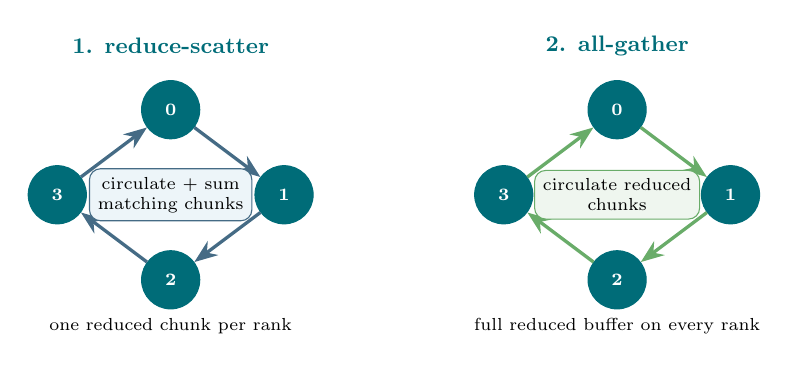
\begin{tikzpicture}[x=1cm,y=1cm,scale=.9,transform shape,every node/.style={font=\scriptsize},rank/.style={circle,draw=accentdark,fill=accentdark,text=white,minimum size=.82cm,font=\scriptsize\bfseries}]
    \begin{scope}[xshift=0cm]
      \node[font=\small\bfseries,text=accentdark] at (2.4,3.9) {1. reduce-scatter};
      \node[rank] (a0) at (2.4,3.0) {0}; \node[rank] (a1) at (4.0,1.8) {1};
      \node[rank] (a2) at (2.4,.6) {2}; \node[rank] (a3) at (.8,1.8) {3};
      \draw[-{Stealth},very thick,themebluedraw] (a0)--(a1);
      \draw[-{Stealth},very thick,themebluedraw] (a1)--(a2);
      \draw[-{Stealth},very thick,themebluedraw] (a2)--(a3);
      \draw[-{Stealth},very thick,themebluedraw] (a3)--(a0);
      \node[draw=themebluedraw,fill=themebluebg,rounded corners,align=center] at (2.4,1.8) {circulate + sum\\matching chunks};
      \node at (2.4,-.05) {one reduced chunk per rank};
    \end{scope}
    \begin{scope}[xshift=6.3cm]
      \node[font=\small\bfseries,text=accentdark] at (2.4,3.9) {2. all-gather};
      \node[rank] (b0) at (2.4,3.0) {0}; \node[rank] (b1) at (4.0,1.8) {1};
      \node[rank] (b2) at (2.4,.6) {2}; \node[rank] (b3) at (.8,1.8) {3};
      \draw[-{Stealth},very thick,successdraw] (b0)--(b1);
      \draw[-{Stealth},very thick,successdraw] (b1)--(b2);
      \draw[-{Stealth},very thick,successdraw] (b2)--(b3);
      \draw[-{Stealth},very thick,successdraw] (b3)--(b0);
      \node[draw=successdraw,fill=successbg,rounded corners,align=center] at (2.4,1.8) {circulate reduced\\chunks};
      \node at (2.4,-.05) {full reduced buffer on every rank};
    \end{scope}
  \end{tikzpicture}
  \vspace{-2pt}
  \begin{block}{Per-rank payload for gradient buffer $S$}
    \centering $2\frac{W-1}{W}S$ bytes, ignoring latency and protocol overhead.
  \end{block}
  \smallsource{Hugging Face Ultra-Scale Playbook}
\end{frame}

\section{Overlap and rank-aware state}

\begin{frame}{Buckets overlap communication with backward}
  Backward produces gradients from later layers first. DDP groups parameters into buckets and launches a collective as each bucket becomes ready.
  \vspace{6pt}
  \begin{center}
  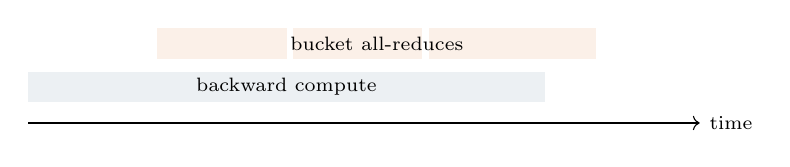
\begin{tikzpicture}[x=.82cm,y=.65cm,every node/.style={font=\scriptsize}]
    \draw[->] (0,0)--(10.4,0) node[right]{time};
    \fill[themebluecard] (0,.4) rectangle (8,1.0);
    \node at (4,.7) {backward compute};
    \fill[warningbg] (2.0,1.25) rectangle (4.0,1.85);
    \fill[warningbg] (4.1,1.25) rectangle (6.1,1.85);
    \fill[warningbg] (6.2,1.25) rectangle (8.8,1.85);
    \node at (5.4,1.55) {bucket all-reduces};
  \end{tikzpicture}
  \end{center}
  \begin{alertblock}{Tail exposure}
    Communication that remains after backward completes is visible step-time overhead.
  \end{alertblock}
\end{frame}

\begin{frame}{Accumulation should synchronize once per update}
  \begin{columns}[c]
    \begin{column}{0.53\linewidth}
      \begin{itemize}
        \setlength{\itemsep}{8pt}
        \item Early micro-steps accumulate locally under \texttt{no\_sync()}.
        \item The final micro-step triggers the bucket all-reduces.
        \item Loss normalization still targets the global mean.
      \end{itemize}
    \end{column}
    \begin{column}{0.43\linewidth}
      \begin{alertblock}{Common waste}
        Synchronizing every micro-step communicates $K$ times for one optimizer update.
      \end{alertblock}
      \begin{block}{Common bug}
        Never synchronizing lets replicas drift immediately after the update.
      \end{block}
    \end{column}
  \end{columns}
\end{frame}

\begin{frame}{Distributed sampling is part of correctness}
  \begin{itemize}
    \setlength{\itemsep}{8pt}
    \item Each rank needs a disjoint subset within an epoch or sampling interval.
    \item All ranks must agree on the shuffle seed and epoch counter.
    \item Dropping or padding the tail changes sample multiplicity.
    \item Resume must restore the sampler's logical position.
  \end{itemize}
  \begin{block}{Fast audit}
    Log sample IDs per rank for a few updates. Check within-step overlap, missing examples, and resume continuity.
  \end{block}
\end{frame}

\begin{frame}{Only some side effects should happen on every rank}
  \small
  \begin{tabular}{lll}
    \toprule
    Action & Every rank? & Reason \\
    \midrule
    forward and backward & yes & local data contribution \\
    optimizer update & yes & replicas remain identical \\
    metric numerator/count & yes & later reduction \\
    console and tracker logging & usually rank 0 & avoid duplicates \\
    full checkpoint publication & coordinated & avoid corruption \\
    validation sampling & sharded or rank 0 & declare aggregation \\
    \bottomrule
  \end{tabular}
\end{frame}

\checkpoint{batch accounting}
  {With $W=8$, micro-batch 2, context 2048, and four accumulated micro-steps, compute tokens per update. How many gradient synchronizations should occur?}

\section{Correctness before scaling}

\begin{frame}{A five-rung correctness ladder}
  \begin{enumerate}
    \setlength{\itemsep}{5pt}
    \item parameters are identical immediately after initialization
    \item one global-batch update matches a single-process reference
    \item parameters remain synchronized after the update
    \item sample IDs show the intended global data coverage
    \item save and resume preserve model, optimizer, RNG, and sampler state
  \end{enumerate}
  \begin{alertblock}{Tolerance is part of the test}
    Reduction order changes floating-point rounding. Define acceptable numerical error rather than demanding bitwise equality by accident.
  \end{alertblock}
\end{frame}

\begin{frame}{Scaling efficiency separates speed from more work}
  \[
    \text{speedup}(W)=\frac{t_1}{t_W},
    \qquad
    \text{efficiency}(W)=\frac{\text{speedup}(W)}{W}
  \]
  \begin{columns}[t]
    \begin{column}{0.47\linewidth}
      \begin{block}{Strong scaling}
        Hold the global batch and work fixed. Ask how much faster the same update becomes.
      \end{block}
    \end{column}
    \begin{column}{0.47\linewidth}
      \begin{block}{Weak scaling}
        Hold work per GPU fixed. Global batch grows with $W$.
      \end{block}
    \end{column}
  \end{columns}
\end{frame}

\begin{frame}{A trace explains poor scaling}
  \begin{itemize}
    \setlength{\itemsep}{7pt}
    \item long exposed collectives suggest insufficient compute overlap or slow links
    \item rank skew suggests data loading, imbalance, or stragglers
    \item many small collectives suggest poor bucketing
    \item gaps before collectives suggest autograd readiness or synchronization barriers
    \item identical time with more GPUs may mean the local batch became too small
  \end{itemize}
\end{frame}

\checkpoint{equivalence failure}
  {A two-GPU run has the expected throughput, but its first update differs sharply from the single-process reference. Give a check order covering initialization, data, loss normalization, reduction, and optimizer state.}

\takeaways
  {DDP is equivalent to a global mean update only when data and normalization invariants hold.}
  {Ring all-reduce spreads bandwidth cost, while buckets hide part of it behind backward.}
  {Sampling, metrics, side effects, and resume logic must all understand rank.}
  {Correctness comparisons come before speedup and efficiency measurements.}
\end{document}
